\documentclass{beamer}
\usepackage[utf8]{inputenc}

\usetheme{Madrid}
\usecolortheme{default}
\usepackage{amsmath,amssymb,amsfonts,amsthm}
\usepackage{txfonts}
\usepackage{tkz-euclide}
\usepackage{listings}
\usepackage{adjustbox}
\usepackage{array}
\usepackage{tabularx}
\usepackage{gvv}
\usepackage{lmodern}
\usepackage{circuitikz}
\usepackage{tikz}
\usepackage{graphicx}

\setbeamertemplate{page number in head/foot}[totalframenumber]

\title{4.4.37}
\date{\today}
\author{EE25BTECH11001 - Aarush Dilawri}

\begin{document}

\frame{\titlepage}


\begin{frame}{Question}
Find the vector equation of the line passing through the point \brak{2,3,-5} and making equal angles with the coordinate axes.
\end{frame}

\begin{frame}{Solution}
Let the line be
\begin{align}
    \vec{x} = \vec{h} + \kappa\vec{m}
\end{align}
where $\vec{m}$ is the direction unit vector of the line, $\vec{h}$ is any given point on the line and $\lvert \kappa \rvert$ is the distance of $\vec{x}$ from $\vec{h}$ along the line.
\end{frame}

\begin{frame}{Solution}
Here,
\begin{align}
    \vec{h} = \myvec{2 \\ 3 \\ -5}
\end{align}
We are given that the line makes equal angles with the coordinate axes. Therefore,
\begin{align}
    \vec{m^T}e_1 = \vec{m^T}e_2 = \vec{m^T}e_3 = \lambda
\end{align}
\end{frame}

\begin{frame}{Solution}
where,
\begin{align}
    \vec{e_1} = \myvec{1 \\ 0 \\ 0}, \quad
    \vec{e_2} = \myvec{0 \\ 1 \\ 0}, \quad
    \vec{e_3} = \myvec{0 \\ 0 \\ 1}
\end{align}
From \brak{0.3},
\begin{align}
    \vec{m^T}\myvec{\vec{e_1} && \vec{e_2} && \vec{e_3}} = \lambda\myvec{1 && 1 && 1}
\end{align}
\end{frame}

\begin{frame}{Solution}
\begin{align}
    \vec{m^T}\myvec{1 && 0 && 0 \\ 0 && 1 && 0 \\ 0 && 0 && 1} = \lambda\myvec{1 && 1 && 1}\\
    \vec{m^T}\vec{I} = \lambda\myvec{1 && 1 && 1}\\
    \vec{m^T} = \lambda\myvec{1 && 1 && 1}
\end{align}
Taking transpose on both sides,
\begin{align}
    \vec{m} = \myvec{\lambda \\ \lambda \\ \lambda}
\end{align}
\end{frame}

\begin{frame}{Solution}
Since,
\begin{align}
    \big\lVert \vec{m} \big\rVert = 1\\
    \lambda = \pm\frac{1}{\sqrt{3}}
\end{align}
Therefore the equation of the line is
\begin{align}
    \vec{x} = \myvec{2 \\ 3 \\ -5} + \kappa\myvec{\tfrac{1}{\sqrt{3}} \\ \tfrac{1}{\sqrt{3}} \\ \tfrac{1}{\sqrt{3}}} 
\end{align}
\end{frame}

\begin{frame}{Figure}
From the figure, it is clearly verified that the theoretical solution matches with the computational solution.
\begin{figure}[h!]
    \centering
    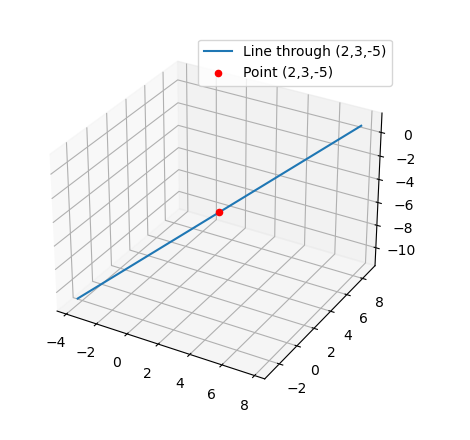
\includegraphics[height=0.5\textheight, keepaspectratio]{figs/fig.png}
    %\caption{Direction and Normal Vectors}
\end{figure}
\end{frame}


% ---------- C CODE ----------
\begin{frame}[fragile]{C Code (code.c)}
\begin{lstlisting}[language=C]
// code.c
#include <stdio.h>
#include <math.h>

// Function to compute m vector (equal angle with axes)
void get_m(double *mx, double *my, double *mz) {
    double val = 1.0 / sqrt(3.0);
    *mx = val;
    *my = val;
    *mz = val;
}
\end{lstlisting}
\end{frame}

\begin{frame}[fragile]{Python Code (code.py)}
\begin{lstlisting}[language=Python]
import numpy as np
import matplotlib.pyplot as plt

# Compute m vector directly
m = np.array([1/np.sqrt(3), 1/np.sqrt(3), 1/np.sqrt(3)])
print("m vector from Python:", m)

# Point through which line passes
P = np.array([2, 3, -5])

# Line: r = P + t*m

\end{lstlisting}
\end{frame}

\begin{frame}[fragile]{Python Code (code.py)}
\begin{lstlisting}[language=Python]
t = np.linspace(-10, 10, 100)
X = P[0] + t * m[0]
Y = P[1] + t * m[1]
Z = P[2] + t * m[2]

# Plot
fig = plt.figure()
ax = fig.add_subplot(111, projection='3d')
ax.plot(X, Y, Z, label="Line through (2,3,-5)")
ax.scatter(P[0], P[1], P[2], color="red", label="Point (2,3,-5)")
ax.legend()
plt.show()
\end{lstlisting}
\end{frame}


\begin{frame}[fragile]{Python Code (nativecode.py)}
\begin{lstlisting}[language=Python]
import ctypes
import numpy as np
import matplotlib.pyplot as plt

# Load the shared object
lib = ctypes.CDLL("./code.so")

# Define the function signature
lib.get_m.argtypes = [ctypes.POINTER(ctypes.c_double),
                      ctypes.POINTER(ctypes.c_double),
                      ctypes.POINTER(ctypes.c_double)]

# Prepare variables
mx = ctypes.c_double()
my = ctypes.c_double()
mz = ctypes.c_double()
\end{lstlisting}
\end{frame}
\begin{frame}[fragile]{Python Code (nativecode.py)}
\begin{lstlisting}[language=Python]
lib.get_m(ctypes.byref(mx), ctypes.byref(my), ctypes.byref(mz))
m = np.array([mx.value, my.value, mz.value])
print("m vector from C:", m)

# Point through which line passes
P = np.array([2, 3, -5])

# Line: r = P + t*m
t = np.linspace(-10, 10, 100)
X = P[0] + t * m[0]
Y = P[1] + t * m[1]
Z = P[2] + t * m[2]
\end{lstlisting}
\end{frame}
\begin{frame}[fragile]{Python Code (nativecode.py)}
\begin{lstlisting}[language=Python]
# Plot
fig = plt.figure()
ax = fig.add_subplot(111, projection='3d')
ax.plot(X, Y, Z, label="Line through (2,3,-5)")
ax.scatter(P[0], P[1], P[2], color="red", label="Point (2,3,-5)")
ax.legend()
plt.show()
\end{lstlisting}
\end{frame}
\end{document}